\subsection{N-Gram language models}
\label{sec:n_gram_language_models}

\subsubsection{Evaluating language models}

We want to know how close $P(s)$ is to $Q(s)$.
We want to calculate the $\mathcal{L}(P,Q)$. The language learning problem is to find $\text{argmin}_Q\mathcal{L}(P,Q)$.
We need to define $\mathcal{L}$ that takes as input two probability distributions on the same set of events and returns a number.
In the '48 Shannon was studying what information a probability distribution carries.
If we have a measure of information, if it does not change the measure is useless. We are interested in changes, in strange
events. We can measure the "interestingness" of something looking at its probability distribution.
Something that is always happening is boring, something that rarely happens is the most interesting.

\begin{figure}[H]
    \centering
    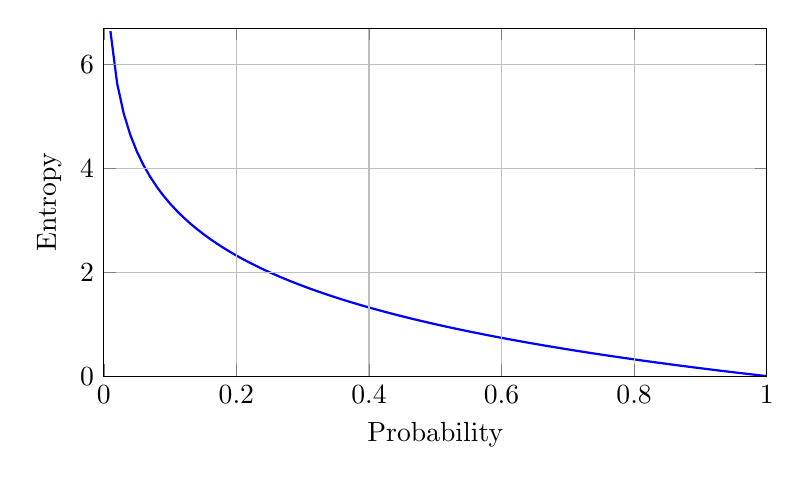
\begin{tikzpicture}
        \begin{axis}[
            xlabel={Probability},
            ylabel={Entropy},
            xmin=0, xmax=1,
            ymin=0, ymax=6.7,
            domain=0.01:1,
            samples=100,
            ytick={0,2,4,6},
            xtick={0,0.2,0.4,0.6,0.8,1},
            grid=major,
            width=10cm,
            height=6cm,
            enlargelimits=false,
            clip=false,
            axis on top,
        ]
        \addplot[blue, thick] {-ln(x)/ln(2)};
        \end{axis}
    \end{tikzpicture}
    \caption{Entropy vs Probability}
    \label{fig:entropy_vs_probability}
\end{figure}

The information content or entropy is defined as
\[
    I[x]=-log(P[x])
\]

We usually calculate the expected value of the information on a 
random variable like this:
\[
    H(X)=E[I(X)]=E[-log(X)]=\sum_{x\in\mathcal{X}}P[x]log(P[x])
\]

If we use the base $e$ we call the unit of measure of $I$ \textbf{nat},
if we use the base 2 we call it \textbf{bit}.

$H$ has some interesting properties:
\begin{itemize}
    \item $H(P) \geq 0$.
    \item $H(P) \leq log(|\mathcal{X}|)$
    \item $H(P)=0 \iff \exists x\in\mathcal{X}:P[x]=1$
    \item $P(P)=log(|\mathcal{X}|) \iff \forall x\in\mathcal{X}:P[x]=\frac{1}{|\mathcal{X}|}$
\end{itemize}

We want to know how much information do we loose if we use
$Q$ instead of $P$.
To do this we use
\[
    H(P,Q)=-\sum_{x\in\mathcal{X}}P[x]log(Q[x])
\]
This is called the \textbf{cross-entropy}.
We leave $P$ because it govern how things actually happen,
we replace $Q$ because that's what governs the information
we have about the world.

(The professor makes an example of what is the interestingness of him
throwing a shoe to a student, even if we don't know the probability
we can approximate an information content that's very high).

With cross entropy we can calculate how much information
we lose (we always lose information with an approximation)
w.r.t. the real world.

The \textbf{Kullback-Leibler divergence} is defined as
\[
    D_{KL}(P||Q)=H(P,Q)-H(P)=-\sum_{x\in\mathcal{X}}P[x]log\left(\frac{Q[x]}{P[x]}\right)
\]

Keep in mind that the divergence is not symmetric:
\[
    D_{KL}(P||Q)\neq D_{KL}(Q||P)
\]
A very important property of the $D_{KL}$ is the
inequality of Gibbs:
\[
    D_{KL}(P||Q)\geq 0
\]

If $P=Q$ then $D_{KL}(P||Q)=0$.

To get back the entropy of sentences we need to normalize
the entropy by the length of the sentence.
$V^+_n$ is the set of all sentences of length $n$,
its cardinality is $|V^+_n|=|V|^n$.
It makes sense to compute the $I[s_n]$ and $H[s_n]$.
The \textbf{entropy rate} is $\bar{H}(s_n)=1/nH[s_n]$.

The entropy of a \textbf{language model} is the limit
of the entropy rate
\[
    H(P)=\lim_{n\rightarrow\infty}\bar{H}(s_n)
\]
And the \textbf{cross-entropy} is
\[
    H(P,Q)=\lim_{n\rightarrow\infty}\frac{1}{n}\sum_{x\in V^+_n}P[s_n]log(Q[s_n])
\]
It makes sense to compute the $D_{KL}$.

The most important theorem in LM theory is the
\textbf{Shannon-McMillan-Breiman theorem}:
Suppose that $P(s)$ and $Q(s)$ are \textbf{good} language models,
knowing the definitions of $V^+,V^+_n,H(P),H(P,Q)$.
$\sigma_n\in V^+_n$ is a single specific element of $V^+_n$.
Then
\[
    H(P,Q)=-\lim_{n\rightarrow\infty}\frac{1}{n}log(Q[\sigma_n])\approxeq
    -\frac{1}{n}log(Q[\sigma_n]) \text{for large enough } n
\]

The first problem that appears is the definition of "\textbf{good}".
In the original theorem stated \textbf{ergodic} and \textbf{stationary}.
\textbf{Stationary} means that the property of the subsequences don't change
independently of their position.
\textbf{Ergodic} basically means that the time average is 
equal to the expectation.
Essentially $n$ should be large enough to see every word in $V$
and appreciate their probability.

Our real value of $n$ is not infinite so we have an approximation.
The sequence $\sigma_n$ that we will use to compute $Q$ is the training corpus $\mathcal{T}$

So given a corpus $\mathcal{T}$ we can compute $H(P,Q)$:
\[
    H(P,Q)=-\frac{1}{T}log(Q[w_1,\dots,w_T])
\]

Remember that the perplexity is defined as
\[
    PP(w_1,\dots,w_T)=exp(log(Q[w_1,\dots,w_T]^{-\frac{1}{T}}))
\]
\[
    =exp(-\frac{1/T}Q[w_1,\dots,w_T])
\]
\[
    =e^{H(P,Q)}
\]

So now we need to solve
\[
    \text{argmin}_Q\mathcal{L}(P,Q)
\]
\[
    =\text{argmin}_Q D_{KL}(P||Q)
\]
\[
    =\text{argmin}_Q H(P,Q)-H(P)
\]
Because $H(P)$ is constant
\[
    =\text{argmin}_Q H(P,Q)
\]
And with the Shannon-McMillan-Breiman theorem we can approximate
to
\[
    \approxeq \text{argmin}_Q -\frac{1}{T}log(Q[w_1,\dots,w_T])
\]

In some scenarios we want to learn 
\[
    P(w|w_1,\dots,w_{n-1})=\begin{cases}
        1 & \text{if } w=w_i\\
        0 & \text{otherwise}
    \end{cases}
\]
This is the word prediction problem.
So it's
\[
    \text{argmax}_Q log(Q[w_T|w_1,\dots,w_{T-1}])
\]

Now we have an estimate of the probability and we can use it
to generate new sentences.

\subsubsection{N-gram models}

An n-gram is a sequence of $n$ words.
The $n$ order Markov assumption is:
Suppose $s\in V^+$, then each word $w\in s$ only depends on the previous $n-1$ words.
\[
    P[s]=P[w_1,\dots,w_n]=\prod_{i=1}^{T}P[w_i|w_{i-1},\dots,w_{i-n+1}]
\]
This is somewhat unrealistic but makes the problem tractable.
Using this assumption we can propose some models:
\begin{itemize}
    \item \textbf{Unigram model}: $P[w_1,\dots,w_k]=\prod_{i=1}^{k}P[w_i]$
    In this case it's very easy to estimate the probabilities with the
    frequencies in the training corpus. This model dos not take into account
    co-occurrences of words.
    \item \textbf{Bigram model}: $P[w_1,\dots,w_k]=\prod_{i=1}^{k}P[w_i|w_{i-1}]$
    \item \textbf{Trigram model}: $P[w_1,\dots,w_k]=\prod_{i=1}^{k}P[w_i|w_{i-1},w_{i-2}]$
    \item and so on...
\end{itemize}

With $n$ growing the training corpus might not contain a certain n-gram.
To solve this we can use \textbf{smoothing} techniques.

Laplace smoothing is the simplest one: "add one to each count".
\[
    P[w_i|\dots]=\frac{C[w_i,\dots]+1}{C[\dots]+|V|}
\]

If we want to use a machine learning model to estimate the 2-gram probabilities we need to
calculate a square matrix $W$ of size $|V|\times|V|$ with all the counts.
To each word $w\in V$ we associate a one-hot vector $x\in Z^{1\times |V|}$.
In $x$ all the elements are 0 except the one corresponding to $w$ (in lexicographic ordering) that is 1.
What is $xW$? It's the row of $W$ corresponding to $w$.

\[
    P[w_i w_j]=\frac{W_ij}{\sum_{j=1}^{|V|}W_ij}
\]

We want to learn this matrix instead of computing it by hand.
We can use a linear layer with weight matrix $\hat{W}$ and learn it, this is an estimate of $W$.
The model is $y=x\hat{W}$. What is $y$? With $\hat{W}$ randomly initialized we get some positive and negative numbers as output.
To get only positive numbers we can use $y=exp(x\hat{W})$. So
$z=(e^{\hat{W}_i1},\dots,e^{\hat{W}_i|V|})$. These are in some way our estimate of the counts.
We call $x\hat{W}$ the \textbf{logits} (logarithm of the counts).
To calculate the probability from the counts we get $P[w_i|w_i]=\frac{z_j}{\sum_{i=1}^{|V|}z_i}$.
This function is called \textbf{softmax}.

Our neural network will be:

\begin{figure}[H]
    \centering
    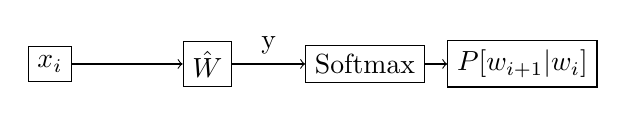
\begin{tikzpicture}[node distance=2cm, auto]
        % Nodes
        \node (input) [draw, rectangle] {$x_i$};
        \node (weights) [draw, rectangle, right of=input] {$\hat{W}$};
        \node (softmax) [draw, rectangle, right of=weights] {Softmax};
        \node (output) [draw, rectangle, right of=softmax] {$P[w_{i+1}|w_i]$};

        % Edges
        \draw[->] (input) -- (weights);
        \draw[->] (weights) -- node[midway, above] {y} (softmax);
        \draw[->] (softmax) -- (output);
    \end{tikzpicture}
    \caption{Neural network for estimating $P[w_{i+1}|w_i]$}
    \label{fig:neural_network}
\end{figure}

We can calculate the loss function
\[
    \mathcal{L}=-\frac{1}{\mathcal{T}}\sum_{i=1}^{|\mathcal{T}|}log(P[w_{i+1}|w_i])
\]

The number of parameters of this model is $|V|^2$. 
If we used a trigram model we would have $|V|^3$ parameters.
This is a lot of parameters, especially considering that $|V|$ is 
in the order of $10^6$. 

A bigram model is quite shitty, and also consumes a lot of memory.